\documentclass[convert]{standalone}

\usepackage{tikz}
\usepackage{standalone}
\usepackage{tikz-feynman}

\begin{document}

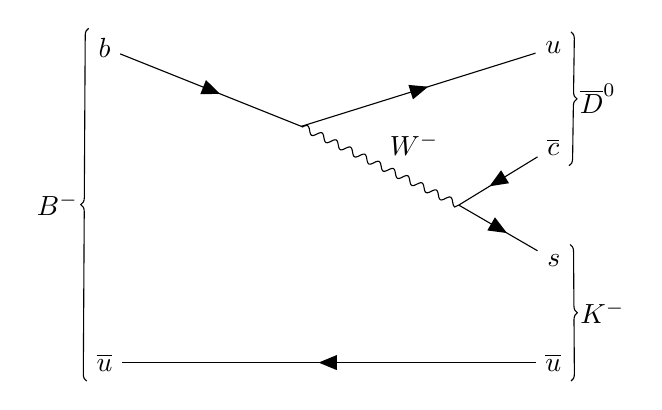
\begin{tikzpicture}
    \begin{feynman}
        \vertex (b) {\(b\)};
        \vertex[below right=1cm and 2.5cm of b] (v1);
        \vertex[below right=1cm and 2cm of v1] (v2);
        \vertex[right=5.7cm of b] (u) {\(u\)};
        \vertex[above right=0.5cm and 1cm of v2] (cBar) {\(\overline{c}\)};
        \vertex[below right=0.5cm and 1cm of v2] (s) {\(s\)};
        \vertex[below=4cm of b] (uBarIn) {\(\overline{u}\)};
        \vertex[right=5.7cm of uBarIn] (uBarOut) {\(\overline{u}\)};
        \diagram* { {[edges=fermion]
                (uBarOut) -- (uBarIn),
                (b) -- (v1) -- (u), (cBar) -- (v2) -- (s)},
        (v1) -- [boson, edge label=\(W^-\)] (v2)
        };
        \draw [decoration={brace}, decorate] (uBarIn.south west) -- (b.north west) node [pos=0.5, left] {\(B^-\)};
        \draw [decoration={brace}, decorate] (s.north east) --  (uBarOut.south east) node [pos=0.5, right] {\(K^-\)};
        \draw [decoration={brace}, decorate] (u.north east) --  (cBar.south east) node [pos=0.5, right] {\(\overline{D}^0\)};
    \end{feynman}
\end{tikzpicture}

\end{document}
